\documentclass[preview=true, border=10pt]{standalone}

\usepackage[compat=1.1.0]{tikz-feynman}

\newcommand{\BdbarToDpiPenguinSize}{6.2}

\begin{document}
	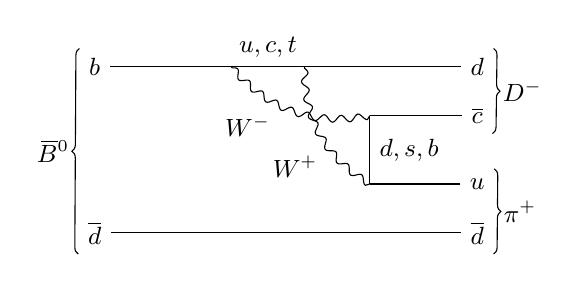
\begin{tikzpicture}
		\begin{feynman}
			\vertex (a1) {\small$b$};
			\vertex[right=\BdbarToDpiPenguinSize*0.28 cm of a1] (a2);
			\vertex[right=\BdbarToDpiPenguinSize*0.15 cm of a2] (a3);
			\vertex[right=\BdbarToDpiPenguinSize*0.32 cm of a3] (a4) {\small$d$};
			\vertex[below=\BdbarToDpiPenguinSize*0.34 cm of a1] (b1) {\small$\overline d$};
			\vertex[below=\BdbarToDpiPenguinSize*0.34 cm of a4] (b2) {\small$\overline d$};
			\vertex[below=\BdbarToDpiPenguinSize*0.10 cm of a4] (c1) {\small$\overline c$};
			\vertex[below=\BdbarToDpiPenguinSize*0.14 cm of c1] (c2) {\small$u$};
			\vertex[left=\BdbarToDpiPenguinSize*0.22 cm of c1] (d1);
			\vertex[left=\BdbarToDpiPenguinSize*0.22 cm of c2] (d2);
			\diagram* {
			(a4) -- [plain] (a3) -- [plain, edge label'={\small$u,c,t$}] (a2) -- [plain] (a1),
			(b1) -- [plain] (b2),
			(c2) -- [plain] (d2) -- [plain, edge label'={\small$d,s,b$}] (d1) -- [plain] (c1),
			(a2) -- [boson, bend right, pos=0.4, edge label'={\small$W^{-}$}] (d1),
			(a3) -- [boson, bend right, pos=0.6, edge label'={\small$W^{+}$}] (d2),
			};
			\draw [decoration={brace}, decorate] (b1.south west) -- (a1.north west) node [pos=0.5, left] {\small$\kern 0.18em\overline{\kern -0.18em B}{}^{0}$};
			\draw [decoration={brace}, decorate] (a4.north east) -- (c1.south east) node [pos=0.5, right] {\small$D^{-}$};
			\draw [decoration={brace}, decorate] (c2.north east) -- (b2.south east) node [pos=0.5, right] {\small$\pi^{+}$};
		\end{feynman}
	\end{tikzpicture}
\end{document}
